\documentclass[1p]{elsarticle_modified}
%\bibliographystyle{elsarticle-num}

%\usepackage[colorlinks]{hyperref}
%\usepackage{abbrmath_seonhwa} %\Abb, \Ascr, \Acal ,\Abf, \Afrak
\usepackage{amsfonts}
\usepackage{amssymb}
\usepackage{amsmath}
\usepackage{amsthm}
\usepackage{scalefnt}
\usepackage{amsbsy}
\usepackage{kotex}
\usepackage{caption}
\usepackage{subfig}
\usepackage{color}
\usepackage{graphicx}
\usepackage{xcolor} %% white, black, red, green, blue, cyan, magenta, yellow
\usepackage{float}
\usepackage{setspace}
\usepackage{hyperref}

\usepackage{tikz}
\usetikzlibrary{arrows}

\usepackage{multirow}
\usepackage{array} % fixed length table
\usepackage{hhline}

%%%%%%%%%%%%%%%%%%%%%
\makeatletter
\renewcommand*\env@matrix[1][\arraystretch]{%
	\edef\arraystretch{#1}%
	\hskip -\arraycolsep
	\let\@ifnextchar\new@ifnextchar
	\array{*\c@MaxMatrixCols c}}
\makeatother %https://tex.stackexchange.com/questions/14071/how-can-i-increase-the-line-spacing-in-a-matrix
%%%%%%%%%%%%%%%

\usepackage[normalem]{ulem}

\newcommand{\msout}[1]{\ifmmode\text{\sout{\ensuremath{#1}}}\else\sout{#1}\fi}
%SOURCE: \msout is \stkout macro in https://tex.stackexchange.com/questions/20609/strikeout-in-math-mode

\newcommand{\cancel}[1]{
	\ifmmode
	{\color{red}\msout{#1}}
	\else
	{\color{red}\sout{#1}}
	\fi
}

\newcommand{\add}[1]{
	{\color{blue}\uwave{#1}}
}

\newcommand{\replace}[2]{
	\ifmmode
	{\color{red}\msout{#1}}{\color{blue}\uwave{#2}}
	\else
	{\color{red}\sout{#1}}{\color{blue}\uwave{#2}}
	\fi
}

\newcommand{\Sol}{\mathcal{S}} %segment
\newcommand{\D}{D} %diagram
\newcommand{\A}{\mathcal{A}} %arc


%%%%%%%%%%%%%%%%%%%%%%%%%%%%%5 test

\def\sl{\operatorname{\textup{SL}}(2,\Cbb)}
\def\psl{\operatorname{\textup{PSL}}(2,\Cbb)}
\def\quan{\mkern 1mu \triangleright \mkern 1mu}

\theoremstyle{definition}
\newtheorem{thm}{Theorem}[section]
\newtheorem{prop}[thm]{Proposition}
\newtheorem{lem}[thm]{Lemma}
\newtheorem{ques}[thm]{Question}
\newtheorem{cor}[thm]{Corollary}
\newtheorem{defn}[thm]{Definition}
\newtheorem{exam}[thm]{Example}
\newtheorem{rmk}[thm]{Remark}
\newtheorem{alg}[thm]{Algorithm}

\newcommand{\I}{\sqrt{-1}}
\begin{document}

%\begin{frontmatter}
%
%\title{Boundary parabolic representations of knots up to 8 crossings}
%
%%% Group authors per affiliation:
%\author{Yunhi Cho} 
%\address{Department of Mathematics, University of Seoul, Seoul, Korea}
%\ead{yhcho@uos.ac.kr}
%
%
%\author{Seonhwa Kim} %\fnref{s_kim}}
%\address{Center for Geometry and Physics, Institute for Basic Science, Pohang, 37673, Korea}
%\ead{ryeona17@ibs.re.kr}
%
%\author{Hyuk Kim}
%\address{Department of Mathematical Sciences, Seoul National University, Seoul 08826, Korea}
%\ead{hyukkim@snu.ac.kr}
%
%\author{Seokbeom Yoon}
%\address{Department of Mathematical Sciences, Seoul National University, Seoul, 08826,  Korea}
%\ead{sbyoon15@snu.ac.kr}
%
%\begin{abstract}
%We find all boundary parabolic representation of knots up to 8 crossings.
%
%\end{abstract}
%\begin{keyword}
%    \MSC[2010] 57M25 
%\end{keyword}
%
%\end{frontmatter}

%\linenumbers
%\tableofcontents
%
\newcommand\colored[1]{\textcolor{white}{\rule[-0.35ex]{0.8em}{1.4ex}}\kern-0.8em\color{red} #1}%
%\newcommand\colored[1]{\textcolor{white}{ #1}\kern-2.17ex	\textcolor{white}{ #1}\kern-1.81ex	\textcolor{white}{ #1}\kern-2.15ex\color{red}#1	}

{\Large $\underline{12n_{0627}~(K12n_{0627})}$}

\setlength{\tabcolsep}{10pt}
\renewcommand{\arraystretch}{1.6}
\vspace{1cm}\begin{tabular}{m{100pt}>{\centering\arraybackslash}m{274pt}}
\multirow{5}{120pt}{
	\centering
	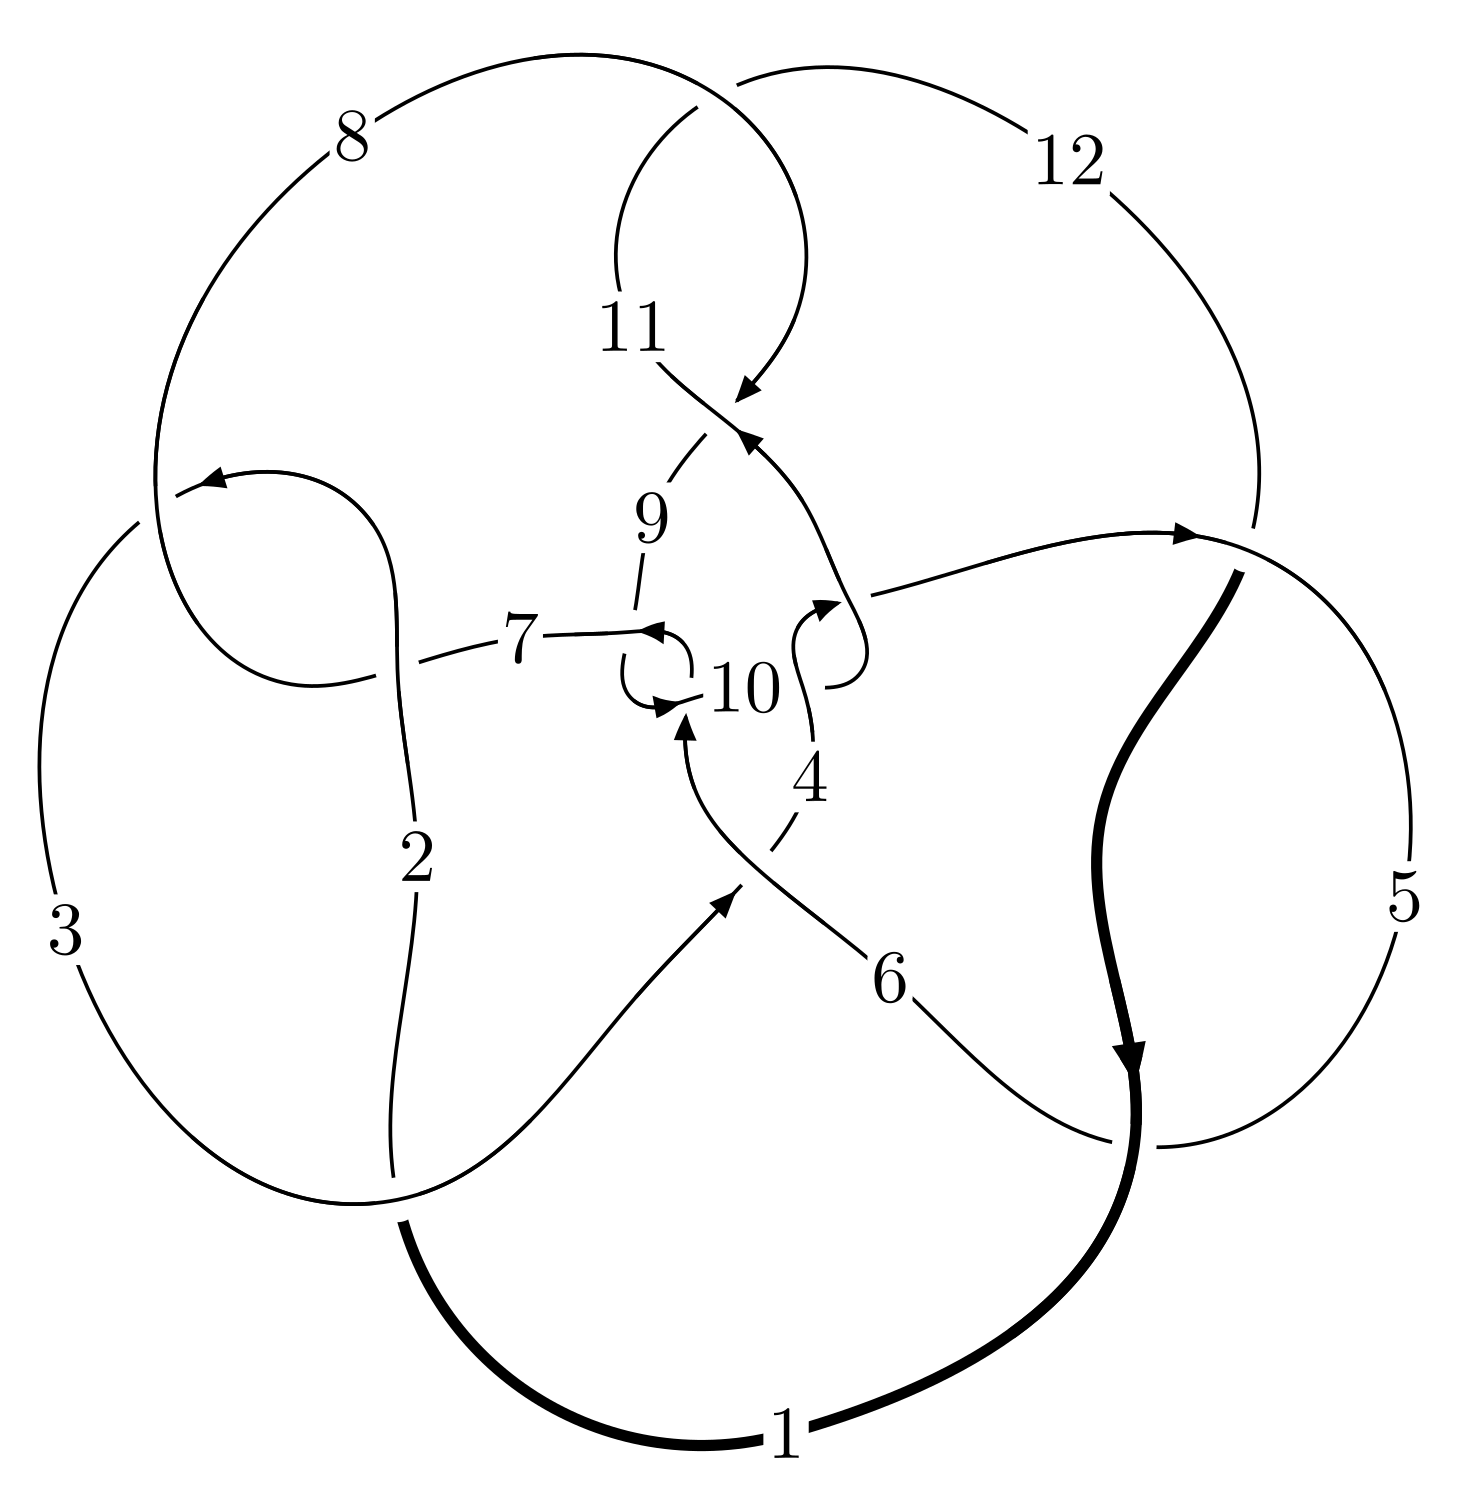
\includegraphics[width=112pt]{../../../GIT/diagram.site/Diagrams/png/2716_12n_0627.png}\\
\ \ \ A knot diagram\footnotemark}&
\allowdisplaybreaks
\textbf{Linearized knot diagam} \\
\cline{2-2}
 &
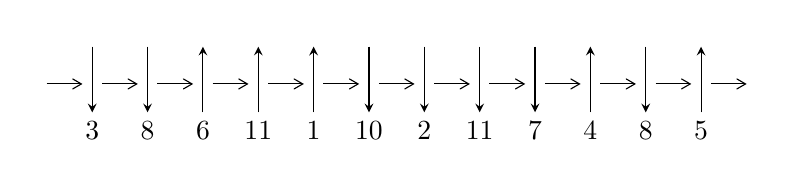
\begin{tikzpicture}[x=20pt, y=17pt]
	% nodes
	\node (C0) at (0, 0) {};
	\node (C1) at (1, 0) {};
	\node (C1U) at (1, +1) {};
	\node (C1D) at (1, -1) {3};

	\node (C2) at (2, 0) {};
	\node (C2U) at (2, +1) {};
	\node (C2D) at (2, -1) {8};

	\node (C3) at (3, 0) {};
	\node (C3U) at (3, +1) {};
	\node (C3D) at (3, -1) {6};

	\node (C4) at (4, 0) {};
	\node (C4U) at (4, +1) {};
	\node (C4D) at (4, -1) {11};

	\node (C5) at (5, 0) {};
	\node (C5U) at (5, +1) {};
	\node (C5D) at (5, -1) {1};

	\node (C6) at (6, 0) {};
	\node (C6U) at (6, +1) {};
	\node (C6D) at (6, -1) {10};

	\node (C7) at (7, 0) {};
	\node (C7U) at (7, +1) {};
	\node (C7D) at (7, -1) {2};

	\node (C8) at (8, 0) {};
	\node (C8U) at (8, +1) {};
	\node (C8D) at (8, -1) {11};

	\node (C9) at (9, 0) {};
	\node (C9U) at (9, +1) {};
	\node (C9D) at (9, -1) {7};

	\node (C10) at (10, 0) {};
	\node (C10U) at (10, +1) {};
	\node (C10D) at (10, -1) {4};

	\node (C11) at (11, 0) {};
	\node (C11U) at (11, +1) {};
	\node (C11D) at (11, -1) {8};

	\node (C12) at (12, 0) {};
	\node (C12U) at (12, +1) {};
	\node (C12D) at (12, -1) {5};
	\node (C13) at (13, 0) {};

	% arrows
	\draw[->,>={angle 60}]
	(C0) edge (C1) (C1) edge (C2) (C2) edge (C3) (C3) edge (C4) (C4) edge (C5) (C5) edge (C6) (C6) edge (C7) (C7) edge (C8) (C8) edge (C9) (C9) edge (C10) (C10) edge (C11) (C11) edge (C12) (C12) edge (C13) ;	\draw[->,>=stealth]
	(C1U) edge (C1D) (C2U) edge (C2D) (C3D) edge (C3U) (C4D) edge (C4U) (C5D) edge (C5U) (C6U) edge (C6D) (C7U) edge (C7D) (C8U) edge (C8D) (C9U) edge (C9D) (C10D) edge (C10U) (C11U) edge (C11D) (C12D) edge (C12U) ;
	\end{tikzpicture} \\
\hhline{~~} \\& 
\textbf{Solving Sequence} \\ \cline{2-2} 
 &
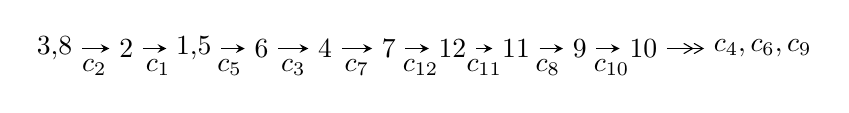
\begin{tikzpicture}[x=23pt, y=7pt]
	% node
	\node (A0) at (-1/8, 0) {3,8};
	\node (A1) at (1, 0) {2};
	\node (A2) at (33/16, 0) {1,5};
	\node (A3) at (25/8, 0) {6};
	\node (A4) at (33/8, 0) {4};
	\node (A5) at (41/8, 0) {7};
	\node (A6) at (49/8, 0) {12};
	\node (A7) at (57/8, 0) {11};
	\node (A8) at (65/8, 0) {9};
	\node (A9) at (73/8, 0) {10};
	\node (C1) at (1/2, -1) {$c_{2}$};
	\node (C2) at (3/2, -1) {$c_{1}$};
	\node (C3) at (21/8, -1) {$c_{5}$};
	\node (C4) at (29/8, -1) {$c_{3}$};
	\node (C5) at (37/8, -1) {$c_{7}$};
	\node (C6) at (45/8, -1) {$c_{12}$};
	\node (C7) at (53/8, -1) {$c_{11}$};
	\node (C8) at (61/8, -1) {$c_{8}$};
	\node (C9) at (69/8, -1) {$c_{10}$};
	\node (A10) at (11, 0) {$c_{4},c_{6},c_{9}$};

	% edge
	\draw[->,>=stealth]	
	(A0) edge (A1) (A1) edge (A2) (A2) edge (A3) (A3) edge (A4) (A4) edge (A5) (A5) edge (A6) (A6) edge (A7) (A7) edge (A8) (A8) edge (A9) ;
	\draw[->>,>={angle 60}]	
	(A9) edge (A10);
\end{tikzpicture} \\ 

\end{tabular} \\

\footnotetext{
The image of knot diagram is generated by the software ``\textbf{Draw programme}" developed by Andrew Bartholomew(\url{http://www.layer8.co.uk/maths/draw/index.htm\#Running-draw}), where we modified some parts for our purpose(\url{https://github.com/CATsTAILs/LinksPainter}).
}\phantom \\ \newline 
\centering \textbf{Ideals for irreducible components\footnotemark of $X_{\text{par}}$} 
 
\begin{align*}
I^u_{1}&=\langle 
-1.15596\times10^{158} u^{88}+1.94754\times10^{158} u^{87}+\cdots+1.32736\times10^{158} b+3.28316\times10^{159},\\
\phantom{I^u_{1}}&\phantom{= \langle  }-1.68579\times10^{158} u^{88}-4.29784\times10^{158} u^{87}+\cdots+6.63682\times10^{158} a-1.27829\times10^{160},\\
\phantom{I^u_{1}}&\phantom{= \langle  }u^{89}- u^{88}+\cdots+14 u-10\rangle \\
I^u_{2}&=\langle 
-348239602 u^{30}+191579437 u^{29}+\cdots+56778667 b+357913195,\\
\phantom{I^u_{2}}&\phantom{= \langle  }24113204363 u^{30}-13246278164 u^{29}+\cdots+1249130674 a-59799820088,\\
\phantom{I^u_{2}}&\phantom{= \langle  }u^{31}-10 u^{29}+\cdots+19 u^2-2\rangle \\
\\
\end{align*}
\raggedright * 2 irreducible components of $\dim_{\mathbb{C}}=0$, with total 120 representations.\\
\footnotetext{All coefficients of polynomials are rational numbers. But the coefficients are sometimes approximated in decimal forms when there is not enough margin.}
\newpage
\renewcommand{\arraystretch}{1}
\centering \section*{I. $I^u_{1}= \langle -1.16\times10^{158} u^{88}+1.95\times10^{158} u^{87}+\cdots+1.33\times10^{158} b+3.28\times10^{159},\;-1.69\times10^{158} u^{88}-4.30\times10^{158} u^{87}+\cdots+6.64\times10^{158} a-1.28\times10^{160},\;u^{89}- u^{88}+\cdots+14 u-10 \rangle$}
\flushleft \textbf{(i) Arc colorings}\\
\begin{tabular}{m{7pt} m{180pt} m{7pt} m{180pt} }
\flushright $a_{3}=$&$\begin{pmatrix}1\\0\end{pmatrix}$ \\
\flushright $a_{8}=$&$\begin{pmatrix}0\\u\end{pmatrix}$ \\
\flushright $a_{2}=$&$\begin{pmatrix}1\\- u^2\end{pmatrix}$ \\
\flushright $a_{1}=$&$\begin{pmatrix}- u^2+1\\- u^2\end{pmatrix}$ \\
\flushright $a_{5}=$&$\begin{pmatrix}0.254006 u^{88}+0.647575 u^{87}+\cdots+7.38084 u+19.2605\\0.870871 u^{88}-1.46722 u^{87}+\cdots+42.4211 u-24.7345\end{pmatrix}$ \\
\flushright $a_{6}=$&$\begin{pmatrix}0.390082 u^{88}+0.0955497 u^{87}+\cdots+14.2030 u+11.8426\\0.488241 u^{88}-1.26681 u^{87}+\cdots+33.9619 u-22.3972\end{pmatrix}$ \\
\flushright $a_{4}=$&$\begin{pmatrix}0.657824 u^{88}+0.241125 u^{87}+\cdots+10.9756 u+16.1052\\-1.86162 u^{88}+2.32381 u^{87}+\cdots-85.2070 u+17.8243\end{pmatrix}$ \\
\flushright $a_{7}=$&$\begin{pmatrix}u\\- u^3+u\end{pmatrix}$ \\
\flushright $a_{12}=$&$\begin{pmatrix}-0.601779 u^{88}+1.28338 u^{87}+\cdots-25.4051 u+11.2090\\2.36178 u^{88}-2.87861 u^{87}+\cdots+87.7562 u-25.7398\end{pmatrix}$ \\
\flushright $a_{11}=$&$\begin{pmatrix}-0.601779 u^{88}+1.28338 u^{87}+\cdots-25.4051 u+11.2090\\2.40515 u^{88}-3.22281 u^{87}+\cdots+103.316 u-32.5558\end{pmatrix}$ \\
\flushright $a_{9}=$&$\begin{pmatrix}0.667097 u^{88}+0.529294 u^{87}+\cdots+4.21757 u+13.2911\\0.694535 u^{88}-0.923902 u^{87}+\cdots-9.67099 u-6.07093\end{pmatrix}$ \\
\flushright $a_{10}=$&$\begin{pmatrix}0.0615361 u^{88}+1.49254 u^{87}+\cdots-11.2489 u+21.9763\\0.289929 u^{88}-0.306028 u^{87}+\cdots-14.0743 u-0.962515\end{pmatrix}$\\&\end{tabular}
\flushleft \textbf{(ii) Obstruction class $= -1$}\\~\\
\flushleft \textbf{(iii) Cusp Shapes $= 3.83185 u^{88}-9.58904 u^{87}+\cdots+2.19711 u-73.4222$}\\~\\
\newpage\renewcommand{\arraystretch}{1}
\flushleft \textbf{(iv) u-Polynomials at the component}\newline \\
\begin{tabular}{m{50pt}|m{274pt}}
Crossings & \hspace{64pt}u-Polynomials at each crossing \\
\hline $$\begin{aligned}c_{1}\end{aligned}$$&$\begin{aligned}
&u^{89}+47 u^{88}+\cdots+2796 u+100
\end{aligned}$\\
\hline $$\begin{aligned}c_{2},c_{7}\end{aligned}$$&$\begin{aligned}
&u^{89}- u^{88}+\cdots+14 u-10
\end{aligned}$\\
\hline $$\begin{aligned}c_{3}\end{aligned}$$&$\begin{aligned}
&u^{89}-2 u^{88}+\cdots+459338 u+255793
\end{aligned}$\\
\hline $$\begin{aligned}c_{4},c_{10}\end{aligned}$$&$\begin{aligned}
&u^{89}+u^{88}+\cdots+119758 u+26770
\end{aligned}$\\
\hline $$\begin{aligned}c_{5},c_{12}\end{aligned}$$&$\begin{aligned}
&u^{89}-2 u^{88}+\cdots+897 u-487
\end{aligned}$\\
\hline $$\begin{aligned}c_{6},c_{9}\end{aligned}$$&$\begin{aligned}
&u^{89}-2 u^{88}+\cdots+39310 u-17077
\end{aligned}$\\
\hline $$\begin{aligned}c_{8},c_{11}\end{aligned}$$&$\begin{aligned}
&u^{89}-6 u^{88}+\cdots-24 u+1
\end{aligned}$\\
\hline
\end{tabular}\\~\\
\newpage\renewcommand{\arraystretch}{1}
\flushleft \textbf{(v) Riley Polynomials at the component}\newline \\
\begin{tabular}{m{50pt}|m{274pt}}
Crossings & \hspace{64pt}Riley Polynomials at each crossing \\
\hline $$\begin{aligned}c_{1}\end{aligned}$$&$\begin{aligned}
&y^{89}+9 y^{88}+\cdots+125616 y-10000
\end{aligned}$\\
\hline $$\begin{aligned}c_{2},c_{7}\end{aligned}$$&$\begin{aligned}
&y^{89}-47 y^{88}+\cdots+2796 y-100
\end{aligned}$\\
\hline $$\begin{aligned}c_{3}\end{aligned}$$&$\begin{aligned}
&y^{89}-66 y^{88}+\cdots+699981667796 y-65430058849
\end{aligned}$\\
\hline $$\begin{aligned}c_{4},c_{10}\end{aligned}$$&$\begin{aligned}
&y^{89}-47 y^{88}+\cdots+24496053724 y-716632900
\end{aligned}$\\
\hline $$\begin{aligned}c_{5},c_{12}\end{aligned}$$&$\begin{aligned}
&y^{89}-42 y^{88}+\cdots+7221321 y-237169
\end{aligned}$\\
\hline $$\begin{aligned}c_{6},c_{9}\end{aligned}$$&$\begin{aligned}
&y^{89}+46 y^{88}+\cdots-11363262354 y-291623929
\end{aligned}$\\
\hline $$\begin{aligned}c_{8},c_{11}\end{aligned}$$&$\begin{aligned}
&y^{89}-58 y^{88}+\cdots+1046 y-1
\end{aligned}$\\
\hline
\end{tabular}\\~\\
\newpage\flushleft \textbf{(vi) Complex Volumes and Cusp Shapes}
$$\begin{array}{c|c|c}  
\text{Solutions to }I^u_{1}& \I (\text{vol} + \sqrt{-1}CS) & \text{Cusp shape}\\
 \hline 
\begin{aligned}
u &= -0.244565 + 0.962025 I \\
a &= \phantom{-}1.53167 - 0.13930 I \\
b &= \phantom{-}0.176114 + 0.504007 I\end{aligned}
 & \phantom{-}1.89844 - 3.40493 I & \phantom{-0.000000 } 0 \\ \hline\begin{aligned}
u &= -0.244565 - 0.962025 I \\
a &= \phantom{-}1.53167 + 0.13930 I \\
b &= \phantom{-}0.176114 - 0.504007 I\end{aligned}
 & \phantom{-}1.89844 + 3.40493 I & \phantom{-0.000000 } 0 \\ \hline\begin{aligned}
u &= \phantom{-}0.933890 + 0.327481 I \\
a &= \phantom{-}0.62035 + 1.46865 I \\
b &= \phantom{-}0.351461 + 1.150610 I\end{aligned}
 & -4.92041 - 1.30903 I & \phantom{-0.000000 } 0 \\ \hline\begin{aligned}
u &= \phantom{-}0.933890 - 0.327481 I \\
a &= \phantom{-}0.62035 - 1.46865 I \\
b &= \phantom{-}0.351461 - 1.150610 I\end{aligned}
 & -4.92041 + 1.30903 I & \phantom{-0.000000 } 0 \\ \hline\begin{aligned}
u &= \phantom{-}0.961254 + 0.394274 I \\
a &= -0.771016 - 0.926200 I \\
b &= -1.13991 + 0.95033 I\end{aligned}
 & \phantom{-}4.21665 - 2.92405 I & \phantom{-0.000000 } 0 \\ \hline\begin{aligned}
u &= \phantom{-}0.961254 - 0.394274 I \\
a &= -0.771016 + 0.926200 I \\
b &= -1.13991 - 0.95033 I\end{aligned}
 & \phantom{-}4.21665 + 2.92405 I & \phantom{-0.000000 } 0 \\ \hline\begin{aligned}
u &= \phantom{-}0.984368 + 0.348236 I \\
a &= -0.171491 - 0.166467 I \\
b &= \phantom{-}0.615879 + 0.898837 I\end{aligned}
 & -0.92696 - 3.77876 I & \phantom{-0.000000 } 0 \\ \hline\begin{aligned}
u &= \phantom{-}0.984368 - 0.348236 I \\
a &= -0.171491 + 0.166467 I \\
b &= \phantom{-}0.615879 - 0.898837 I\end{aligned}
 & -0.92696 + 3.77876 I & \phantom{-0.000000 } 0 \\ \hline\begin{aligned}
u &= -0.930123 + 0.518617 I \\
a &= -0.526672 + 0.968906 I \\
b &= -0.159656 - 0.114899 I\end{aligned}
 & \phantom{-}5.18137 + 2.01747 I & \phantom{-0.000000 } 0 \\ \hline\begin{aligned}
u &= -0.930123 - 0.518617 I \\
a &= -0.526672 - 0.968906 I \\
b &= -0.159656 + 0.114899 I\end{aligned}
 & \phantom{-}5.18137 - 2.01747 I & \phantom{-0.000000 } 0\\
 \hline 
 \end{array}$$\newpage$$\begin{array}{c|c|c}  
\text{Solutions to }I^u_{1}& \I (\text{vol} + \sqrt{-1}CS) & \text{Cusp shape}\\
 \hline 
\begin{aligned}
u &= -1.006170 + 0.430405 I \\
a &= -0.438623 + 0.856778 I \\
b &= -2.20252 + 1.49810 I\end{aligned}
 & -2.68981 + 4.03468 I & \phantom{-0.000000 } 0 \\ \hline\begin{aligned}
u &= -1.006170 - 0.430405 I \\
a &= -0.438623 - 0.856778 I \\
b &= -2.20252 - 1.49810 I\end{aligned}
 & -2.68981 - 4.03468 I & \phantom{-0.000000 } 0 \\ \hline\begin{aligned}
u &= \phantom{-}1.039120 + 0.367975 I \\
a &= -0.563115 - 0.858898 I \\
b &= -2.46344 - 1.22813 I\end{aligned}
 & -1.38793 + 2.34054 I & \phantom{-0.000000 } 0 \\ \hline\begin{aligned}
u &= \phantom{-}1.039120 - 0.367975 I \\
a &= -0.563115 + 0.858898 I \\
b &= -2.46344 + 1.22813 I\end{aligned}
 & -1.38793 - 2.34054 I & \phantom{-0.000000 } 0 \\ \hline\begin{aligned}
u &= -0.725494 + 0.521426 I \\
a &= -0.89511 + 1.20991 I \\
b &= -1.47632 + 0.97253 I\end{aligned}
 & \phantom{-}5.84354 + 2.20534 I & \phantom{-0.000000 } 0 \\ \hline\begin{aligned}
u &= -0.725494 - 0.521426 I \\
a &= -0.89511 - 1.20991 I \\
b &= -1.47632 - 0.97253 I\end{aligned}
 & \phantom{-}5.84354 - 2.20534 I & \phantom{-0.000000 } 0 \\ \hline\begin{aligned}
u &= \phantom{-}1.007390 + 0.511262 I \\
a &= -0.398190 - 1.199040 I \\
b &= -0.46816 - 1.60706 I\end{aligned}
 & -2.16350 - 1.93019 I & \phantom{-0.000000 } 0 \\ \hline\begin{aligned}
u &= \phantom{-}1.007390 - 0.511262 I \\
a &= -0.398190 + 1.199040 I \\
b &= -0.46816 + 1.60706 I\end{aligned}
 & -2.16350 + 1.93019 I & \phantom{-0.000000 } 0 \\ \hline\begin{aligned}
u &= \phantom{-}0.385380 + 1.077170 I \\
a &= -1.57779 + 0.35617 I \\
b &= -0.413188 + 0.978791 I\end{aligned}
 & \phantom{-}4.95394 + 10.81390 I & \phantom{-0.000000 } 0 \\ \hline\begin{aligned}
u &= \phantom{-}0.385380 - 1.077170 I \\
a &= -1.57779 - 0.35617 I \\
b &= -0.413188 - 0.978791 I\end{aligned}
 & \phantom{-}4.95394 - 10.81390 I & \phantom{-0.000000 } 0\\
 \hline 
 \end{array}$$\newpage$$\begin{array}{c|c|c}  
\text{Solutions to }I^u_{1}& \I (\text{vol} + \sqrt{-1}CS) & \text{Cusp shape}\\
 \hline 
\begin{aligned}
u &= -0.550489 + 1.004510 I \\
a &= -1.115950 - 0.400395 I \\
b &= -0.275463 - 1.059970 I\end{aligned}
 & \phantom{-}1.00206 - 3.24358 I & \phantom{-0.000000 } 0 \\ \hline\begin{aligned}
u &= -0.550489 - 1.004510 I \\
a &= -1.115950 + 0.400395 I \\
b &= -0.275463 + 1.059970 I\end{aligned}
 & \phantom{-}1.00206 + 3.24358 I & \phantom{-0.000000 } 0 \\ \hline\begin{aligned}
u &= \phantom{-}0.193852 + 0.828020 I \\
a &= \phantom{-}1.149260 - 0.120601 I \\
b &= \phantom{-}0.025384 - 0.661444 I\end{aligned}
 & \phantom{-}0.840044 + 0.487278 I & \phantom{-}3.75141 + 1.24704 I \\ \hline\begin{aligned}
u &= \phantom{-}0.193852 - 0.828020 I \\
a &= \phantom{-}1.149260 + 0.120601 I \\
b &= \phantom{-}0.025384 + 0.661444 I\end{aligned}
 & \phantom{-}0.840044 - 0.487278 I & \phantom{-}3.75141 - 1.24704 I \\ \hline\begin{aligned}
u &= \phantom{-}0.755613 + 0.358139 I \\
a &= -0.30612 - 1.66985 I \\
b &= -2.39351 - 0.85784 I\end{aligned}
 & \phantom{-}4.96330 - 0.31485 I & \phantom{-}3.79476 - 1.00054 I \\ \hline\begin{aligned}
u &= \phantom{-}0.755613 - 0.358139 I \\
a &= -0.30612 + 1.66985 I \\
b &= -2.39351 + 0.85784 I\end{aligned}
 & \phantom{-}4.96330 + 0.31485 I & \phantom{-}3.79476 + 1.00054 I \\ \hline\begin{aligned}
u &= \phantom{-}0.670677 + 0.495093 I \\
a &= -1.56847 - 0.88463 I \\
b &= \phantom{-}0.036229 + 0.286376 I\end{aligned}
 & -1.01560 - 2.22245 I & \phantom{-}1.10851 + 6.52104 I \\ \hline\begin{aligned}
u &= \phantom{-}0.670677 - 0.495093 I \\
a &= -1.56847 + 0.88463 I \\
b &= \phantom{-}0.036229 - 0.286376 I\end{aligned}
 & -1.01560 + 2.22245 I & \phantom{-}1.10851 - 6.52104 I \\ \hline\begin{aligned}
u &= -1.047730 + 0.520787 I \\
a &= -0.428255 + 1.175960 I \\
b &= -0.149308 + 1.361530 I\end{aligned}
 & -0.36097 + 8.88020 I & \phantom{-0.000000 } 0 \\ \hline\begin{aligned}
u &= -1.047730 - 0.520787 I \\
a &= -0.428255 - 1.175960 I \\
b &= -0.149308 - 1.361530 I\end{aligned}
 & -0.36097 - 8.88020 I & \phantom{-0.000000 } 0\\
 \hline 
 \end{array}$$\newpage$$\begin{array}{c|c|c}  
\text{Solutions to }I^u_{1}& \I (\text{vol} + \sqrt{-1}CS) & \text{Cusp shape}\\
 \hline 
\begin{aligned}
u &= \phantom{-}0.135466 + 0.812923 I \\
a &= \phantom{-}0.0767182 - 0.0995383 I \\
b &= \phantom{-}0.694405 + 0.225698 I\end{aligned}
 & \phantom{-}7.98738 + 2.98075 I & \phantom{-}6.24007 - 3.70589 I \\ \hline\begin{aligned}
u &= \phantom{-}0.135466 - 0.812923 I \\
a &= \phantom{-}0.0767182 + 0.0995383 I \\
b &= \phantom{-}0.694405 - 0.225698 I\end{aligned}
 & \phantom{-}7.98738 - 2.98075 I & \phantom{-}6.24007 + 3.70589 I \\ \hline\begin{aligned}
u &= -1.093460 + 0.434573 I \\
a &= \phantom{-}0.091617 + 0.515957 I \\
b &= -0.56916 + 2.20034 I\end{aligned}
 & \phantom{-}6.64364 + 5.23146 I & \phantom{-0.000000 } 0 \\ \hline\begin{aligned}
u &= -1.093460 - 0.434573 I \\
a &= \phantom{-}0.091617 - 0.515957 I \\
b &= -0.56916 - 2.20034 I\end{aligned}
 & \phantom{-}6.64364 - 5.23146 I & \phantom{-0.000000 } 0 \\ \hline\begin{aligned}
u &= \phantom{-}1.184860 + 0.009536 I \\
a &= -0.068200 + 1.014210 I \\
b &= \phantom{-}0.194397 + 0.996138 I\end{aligned}
 & -6.31122 - 1.42992 I & \phantom{-0.000000 } 0 \\ \hline\begin{aligned}
u &= \phantom{-}1.184860 - 0.009536 I \\
a &= -0.068200 - 1.014210 I \\
b &= \phantom{-}0.194397 - 0.996138 I\end{aligned}
 & -6.31122 + 1.42992 I & \phantom{-0.000000 } 0 \\ \hline\begin{aligned}
u &= -1.037570 + 0.577206 I \\
a &= \phantom{-}0.264692 - 1.356690 I \\
b &= \phantom{-}1.86795 - 1.60205 I\end{aligned}
 & -2.93078 + 4.54020 I & \phantom{-0.000000 } 0 \\ \hline\begin{aligned}
u &= -1.037570 - 0.577206 I \\
a &= \phantom{-}0.264692 + 1.356690 I \\
b &= \phantom{-}1.86795 + 1.60205 I\end{aligned}
 & -2.93078 - 4.54020 I & \phantom{-0.000000 } 0 \\ \hline\begin{aligned}
u &= \phantom{-}1.069300 + 0.535238 I \\
a &= -0.212727 - 0.410896 I \\
b &= -1.03867 - 1.58194 I\end{aligned}
 & \phantom{-}7.46229 - 1.93692 I & \phantom{-0.000000 } 0 \\ \hline\begin{aligned}
u &= \phantom{-}1.069300 - 0.535238 I \\
a &= -0.212727 + 0.410896 I \\
b &= -1.03867 + 1.58194 I\end{aligned}
 & \phantom{-}7.46229 + 1.93692 I & \phantom{-0.000000 } 0\\
 \hline 
 \end{array}$$\newpage$$\begin{array}{c|c|c}  
\text{Solutions to }I^u_{1}& \I (\text{vol} + \sqrt{-1}CS) & \text{Cusp shape}\\
 \hline 
\begin{aligned}
u &= -0.515011 + 0.603128 I \\
a &= \phantom{-}1.64276 - 0.39430 I \\
b &= \phantom{-}0.492067 + 0.826898 I\end{aligned}
 & -1.41949 + 0.21530 I & -1.33212 - 0.94894 I \\ \hline\begin{aligned}
u &= -0.515011 - 0.603128 I \\
a &= \phantom{-}1.64276 + 0.39430 I \\
b &= \phantom{-}0.492067 - 0.826898 I\end{aligned}
 & -1.41949 - 0.21530 I & -1.33212 + 0.94894 I \\ \hline\begin{aligned}
u &= -0.864934 + 0.865784 I \\
a &= \phantom{-}0.37365 + 1.86763 I \\
b &= -0.69775 + 1.96712 I\end{aligned}
 & \phantom{-}7.10528 - 0.44632 I & \phantom{-0.000000 } 0 \\ \hline\begin{aligned}
u &= -0.864934 - 0.865784 I \\
a &= \phantom{-}0.37365 - 1.86763 I \\
b &= -0.69775 - 1.96712 I\end{aligned}
 & \phantom{-}7.10528 + 0.44632 I & \phantom{-0.000000 } 0 \\ \hline\begin{aligned}
u &= -1.178880 + 0.353943 I \\
a &= \phantom{-}0.754751 - 1.024090 I \\
b &= \phantom{-}0.733978 - 1.009140 I\end{aligned}
 & -3.35558 - 1.16932 I & \phantom{-0.000000 } 0 \\ \hline\begin{aligned}
u &= -1.178880 - 0.353943 I \\
a &= \phantom{-}0.754751 + 1.024090 I \\
b &= \phantom{-}0.733978 + 1.009140 I\end{aligned}
 & -3.35558 + 1.16932 I & \phantom{-0.000000 } 0 \\ \hline\begin{aligned}
u &= \phantom{-}1.125660 + 0.509560 I \\
a &= \phantom{-}0.137200 + 1.400810 I \\
b &= \phantom{-}1.92996 + 2.24231 I\end{aligned}
 & -2.31939 - 9.19141 I & \phantom{-0.000000 } 0 \\ \hline\begin{aligned}
u &= \phantom{-}1.125660 - 0.509560 I \\
a &= \phantom{-}0.137200 - 1.400810 I \\
b &= \phantom{-}1.92996 - 2.24231 I\end{aligned}
 & -2.31939 + 9.19141 I & \phantom{-0.000000 } 0 \\ \hline\begin{aligned}
u &= -0.939369 + 0.825652 I \\
a &= -1.75974 - 1.01547 I \\
b &= -0.34731 - 1.89934 I\end{aligned}
 & \phantom{-}6.86423 + 6.71990 I & \phantom{-0.000000 } 0 \\ \hline\begin{aligned}
u &= -0.939369 - 0.825652 I \\
a &= -1.75974 + 1.01547 I \\
b &= -0.34731 + 1.89934 I\end{aligned}
 & \phantom{-}6.86423 - 6.71990 I & \phantom{-0.000000 } 0\\
 \hline 
 \end{array}$$\newpage$$\begin{array}{c|c|c}  
\text{Solutions to }I^u_{1}& \I (\text{vol} + \sqrt{-1}CS) & \text{Cusp shape}\\
 \hline 
\begin{aligned}
u &= -0.704939 + 0.128997 I \\
a &= \phantom{-}0.678583 - 0.630657 I \\
b &= \phantom{-}0.201233 + 0.306478 I\end{aligned}
 & -1.278980 + 0.553347 I & -4.94268 - 0.11935 I \\ \hline\begin{aligned}
u &= -0.704939 - 0.128997 I \\
a &= \phantom{-}0.678583 + 0.630657 I \\
b &= \phantom{-}0.201233 - 0.306478 I\end{aligned}
 & -1.278980 - 0.553347 I & -4.94268 + 0.11935 I \\ \hline\begin{aligned}
u &= -0.502799 + 0.482734 I \\
a &= -1.90347 + 1.26712 I \\
b &= -0.306144 + 0.452430 I\end{aligned}
 & \phantom{-}1.30667 - 4.62534 I & \phantom{-}2.58741 + 1.79100 I \\ \hline\begin{aligned}
u &= -0.502799 - 0.482734 I \\
a &= -1.90347 - 1.26712 I \\
b &= -0.306144 - 0.452430 I\end{aligned}
 & \phantom{-}1.30667 + 4.62534 I & \phantom{-}2.58741 - 1.79100 I \\ \hline\begin{aligned}
u &= \phantom{-}1.185270 + 0.561749 I \\
a &= \phantom{-}0.106817 + 0.932579 I \\
b &= \phantom{-}1.35872 + 1.78506 I\end{aligned}
 & -2.03233 - 5.61518 I & \phantom{-0.000000 } 0 \\ \hline\begin{aligned}
u &= \phantom{-}1.185270 - 0.561749 I \\
a &= \phantom{-}0.106817 - 0.932579 I \\
b &= \phantom{-}1.35872 - 1.78506 I\end{aligned}
 & -2.03233 + 5.61518 I & \phantom{-0.000000 } 0 \\ \hline\begin{aligned}
u &= \phantom{-}0.462387 + 0.498609 I \\
a &= -0.355623 - 0.428534 I \\
b &= \phantom{-}1.184450 + 0.682440 I\end{aligned}
 & \phantom{-}9.29816 - 2.41390 I & \phantom{-}1.98968 + 2.16516 I \\ \hline\begin{aligned}
u &= \phantom{-}0.462387 - 0.498609 I \\
a &= -0.355623 + 0.428534 I \\
b &= \phantom{-}1.184450 - 0.682440 I\end{aligned}
 & \phantom{-}9.29816 + 2.41390 I & \phantom{-}1.98968 - 2.16516 I \\ \hline\begin{aligned}
u &= \phantom{-}1.187720 + 0.576982 I \\
a &= -0.0159480 - 0.0353645 I \\
b &= -0.578942 - 0.722269 I\end{aligned}
 & \phantom{-}5.01786 - 8.11410 I & \phantom{-0.000000 } 0 \\ \hline\begin{aligned}
u &= \phantom{-}1.187720 - 0.576982 I \\
a &= -0.0159480 + 0.0353645 I \\
b &= -0.578942 + 0.722269 I\end{aligned}
 & \phantom{-}5.01786 + 8.11410 I & \phantom{-0.000000 } 0\\
 \hline 
 \end{array}$$\newpage$$\begin{array}{c|c|c}  
\text{Solutions to }I^u_{1}& \I (\text{vol} + \sqrt{-1}CS) & \text{Cusp shape}\\
 \hline 
\begin{aligned}
u &= \phantom{-}0.809665 + 1.047990 I \\
a &= -0.578466 + 1.211320 I \\
b &= \phantom{-}0.20865 + 1.46420 I\end{aligned}
 & \phantom{-}7.99506 - 3.76404 I & \phantom{-0.000000 } 0 \\ \hline\begin{aligned}
u &= \phantom{-}0.809665 - 1.047990 I \\
a &= -0.578466 - 1.211320 I \\
b &= \phantom{-}0.20865 - 1.46420 I\end{aligned}
 & \phantom{-}7.99506 + 3.76404 I & \phantom{-0.000000 } 0 \\ \hline\begin{aligned}
u &= -1.297580 + 0.343196 I \\
a &= \phantom{-}0.265023 - 0.728750 I \\
b &= -0.019555 - 0.999504 I\end{aligned}
 & -3.72640 + 3.60063 I & \phantom{-0.000000 } 0 \\ \hline\begin{aligned}
u &= -1.297580 - 0.343196 I \\
a &= \phantom{-}0.265023 + 0.728750 I \\
b &= -0.019555 + 0.999504 I\end{aligned}
 & -3.72640 - 3.60063 I & \phantom{-0.000000 } 0 \\ \hline\begin{aligned}
u &= -1.210270 + 0.608884 I \\
a &= \phantom{-}0.366434 - 1.056420 I \\
b &= \phantom{-}1.51925 - 1.86407 I\end{aligned}
 & -1.01252 + 9.05504 I & \phantom{-0.000000 } 0 \\ \hline\begin{aligned}
u &= -1.210270 - 0.608884 I \\
a &= \phantom{-}0.366434 + 1.056420 I \\
b &= \phantom{-}1.51925 + 1.86407 I\end{aligned}
 & -1.01252 - 9.05504 I & \phantom{-0.000000 } 0 \\ \hline\begin{aligned}
u &= -1.145810 + 0.725166 I \\
a &= \phantom{-}0.081475 + 1.179080 I \\
b &= -1.23733 + 1.76256 I\end{aligned}
 & -0.87540 + 9.52648 I & \phantom{-0.000000 } 0 \\ \hline\begin{aligned}
u &= -1.145810 - 0.725166 I \\
a &= \phantom{-}0.081475 - 1.179080 I \\
b &= -1.23733 - 1.76256 I\end{aligned}
 & -0.87540 - 9.52648 I & \phantom{-0.000000 } 0 \\ \hline\begin{aligned}
u &= \phantom{-}0.119389 + 0.627414 I \\
a &= \phantom{-}2.62220 - 0.47010 I \\
b &= \phantom{-}0.273086 - 0.906877 I\end{aligned}
 & \phantom{-}0.32407 + 4.80711 I & \phantom{-}2.84174 - 5.69896 I \\ \hline\begin{aligned}
u &= \phantom{-}0.119389 - 0.627414 I \\
a &= \phantom{-}2.62220 + 0.47010 I \\
b &= \phantom{-}0.273086 + 0.906877 I\end{aligned}
 & \phantom{-}0.32407 - 4.80711 I & \phantom{-}2.84174 + 5.69896 I\\
 \hline 
 \end{array}$$\newpage$$\begin{array}{c|c|c}  
\text{Solutions to }I^u_{1}& \I (\text{vol} + \sqrt{-1}CS) & \text{Cusp shape}\\
 \hline 
\begin{aligned}
u &= \phantom{-}1.019810 + 0.909269 I \\
a &= \phantom{-}0.814306 - 1.101550 I \\
b &= -0.26325 - 1.57950 I\end{aligned}
 & \phantom{-}7.32281 - 3.25014 I & \phantom{-0.000000 } 0 \\ \hline\begin{aligned}
u &= \phantom{-}1.019810 - 0.909269 I \\
a &= \phantom{-}0.814306 + 1.101550 I \\
b &= -0.26325 + 1.57950 I\end{aligned}
 & \phantom{-}7.32281 + 3.25014 I & \phantom{-0.000000 } 0 \\ \hline\begin{aligned}
u &= -1.267540 + 0.515469 I \\
a &= \phantom{-}0.124014 + 0.094273 I \\
b &= \phantom{-}0.062531 + 0.820397 I\end{aligned}
 & \phantom{-}4.05888 + 1.69142 I & \phantom{-0.000000 } 0 \\ \hline\begin{aligned}
u &= -1.267540 - 0.515469 I \\
a &= \phantom{-}0.124014 - 0.094273 I \\
b &= \phantom{-}0.062531 - 0.820397 I\end{aligned}
 & \phantom{-}4.05888 - 1.69142 I & \phantom{-0.000000 } 0 \\ \hline\begin{aligned}
u &= -0.571300 + 0.255504 I \\
a &= -0.152207 + 1.389420 I \\
b &= \phantom{-}0.055604 - 0.780948 I\end{aligned}
 & -1.30408 - 0.70841 I & -3.23715 - 2.79209 I \\ \hline\begin{aligned}
u &= -0.571300 - 0.255504 I \\
a &= -0.152207 - 1.389420 I \\
b &= \phantom{-}0.055604 + 0.780948 I\end{aligned}
 & -1.30408 + 0.70841 I & -3.23715 + 2.79209 I \\ \hline\begin{aligned}
u &= \phantom{-}1.225220 + 0.689448 I \\
a &= -0.069523 - 1.329850 I \\
b &= -1.36230 - 2.11676 I\end{aligned}
 & \phantom{-}2.3330 - 17.1358 I & \phantom{-0.000000 } 0 \\ \hline\begin{aligned}
u &= \phantom{-}1.225220 - 0.689448 I \\
a &= -0.069523 + 1.329850 I \\
b &= -1.36230 + 2.11676 I\end{aligned}
 & \phantom{-}2.3330 + 17.1358 I & \phantom{-0.000000 } 0 \\ \hline\begin{aligned}
u &= -0.535112 + 0.234522 I \\
a &= -0.662387 + 0.280870 I \\
b &= \phantom{-}1.93398 - 0.90821 I\end{aligned}
 & \phantom{-}8.70160 - 1.90871 I & \phantom{-}7.78540 + 9.95719 I \\ \hline\begin{aligned}
u &= -0.535112 - 0.234522 I \\
a &= -0.662387 - 0.280870 I \\
b &= \phantom{-}1.93398 + 0.90821 I\end{aligned}
 & \phantom{-}8.70160 + 1.90871 I & \phantom{-}7.78540 - 9.95719 I\\
 \hline 
 \end{array}$$\newpage$$\begin{array}{c|c|c}  
\text{Solutions to }I^u_{1}& \I (\text{vol} + \sqrt{-1}CS) & \text{Cusp shape}\\
 \hline 
\begin{aligned}
u &= \phantom{-}0.258887 + 0.501698 I \\
a &= \phantom{-}0.645831 - 0.321842 I \\
b &= -0.399572 - 0.528257 I\end{aligned}
 & \phantom{-}1.169890 + 0.562593 I & \phantom{-}6.08302 - 1.22520 I \\ \hline\begin{aligned}
u &= \phantom{-}0.258887 - 0.501698 I \\
a &= \phantom{-}0.645831 + 0.321842 I \\
b &= -0.399572 + 0.528257 I\end{aligned}
 & \phantom{-}1.169890 - 0.562593 I & \phantom{-}6.08302 + 1.22520 I \\ \hline\begin{aligned}
u &= \phantom{-}1.40041 + 0.31914 I \\
a &= \phantom{-}0.425074 + 0.891756 I \\
b &= \phantom{-}0.47358 + 1.45542 I\end{aligned}
 & -3.47015 - 1.06999 I & \phantom{-0.000000 } 0 \\ \hline\begin{aligned}
u &= \phantom{-}1.40041 - 0.31914 I \\
a &= \phantom{-}0.425074 - 0.891756 I \\
b &= \phantom{-}0.47358 - 1.45542 I\end{aligned}
 & -3.47015 + 1.06999 I & \phantom{-0.000000 } 0 \\ \hline\begin{aligned}
u &= -1.50427 + 0.13904 I \\
a &= -0.652895 + 0.680071 I \\
b &= -0.576514 + 0.878599 I\end{aligned}
 & -1.87227 - 6.46093 I & \phantom{-0.000000 } 0 \\ \hline\begin{aligned}
u &= -1.50427 - 0.13904 I \\
a &= -0.652895 - 0.680071 I \\
b &= -0.576514 - 0.878599 I\end{aligned}
 & -1.87227 + 6.46093 I & \phantom{-0.000000 } 0 \\ \hline\begin{aligned}
u &= \phantom{-}0.444561 + 0.091212 I \\
a &= \phantom{-}0.83158 - 3.45351 I \\
b &= -0.793166 + 1.093540 I\end{aligned}
 & \phantom{-}0.70679 - 4.99686 I & \phantom{-}6.49732 + 8.11595 I \\ \hline\begin{aligned}
u &= \phantom{-}0.444561 - 0.091212 I \\
a &= \phantom{-}0.83158 + 3.45351 I \\
b &= -0.793166 - 1.093540 I\end{aligned}
 & \phantom{-}0.70679 + 4.99686 I & \phantom{-}6.49732 - 8.11595 I \\ \hline\begin{aligned}
u &= \phantom{-}1.62650\phantom{ +0.000000I} \\
a &= -0.224051\phantom{ +0.000000I} \\
b &= -0.115481\phantom{ +0.000000I}\end{aligned}
 & -7.34147\phantom{ +0.000000I} & \phantom{-0.000000 } 0\\
 \hline 
 \end{array}$$\newpage\newpage\renewcommand{\arraystretch}{1}
\centering \section*{II. $I^u_{2}= \langle -3.48\times10^{8} u^{30}+1.92\times10^{8} u^{29}+\cdots+5.68\times10^{7} b+3.58\times10^{8},\;2.41\times10^{10} u^{30}-1.32\times10^{10} u^{29}+\cdots+1.25\times10^{9} a-5.98\times10^{10},\;u^{31}-10 u^{29}+\cdots+19 u^2-2 \rangle$}
\flushleft \textbf{(i) Arc colorings}\\
\begin{tabular}{m{7pt} m{180pt} m{7pt} m{180pt} }
\flushright $a_{3}=$&$\begin{pmatrix}1\\0\end{pmatrix}$ \\
\flushright $a_{8}=$&$\begin{pmatrix}0\\u\end{pmatrix}$ \\
\flushright $a_{2}=$&$\begin{pmatrix}1\\- u^2\end{pmatrix}$ \\
\flushright $a_{1}=$&$\begin{pmatrix}- u^2+1\\- u^2\end{pmatrix}$ \\
\flushright $a_{5}=$&$\begin{pmatrix}-19.3040 u^{30}+10.6044 u^{29}+\cdots-92.5487 u+47.8731\\6.13328 u^{30}-3.37414 u^{29}+\cdots+28.2670 u-6.30366\end{pmatrix}$ \\
\flushright $a_{6}=$&$\begin{pmatrix}-21.3460 u^{30}+13.6987 u^{29}+\cdots-107.471 u+61.2222\\7.93390 u^{30}-4.43203 u^{29}+\cdots+35.9523 u-14.6081\end{pmatrix}$ \\
\flushright $a_{4}=$&$\begin{pmatrix}-19.3040 u^{30}+11.6044 u^{29}+\cdots-92.5487 u+48.8731\\8.67259 u^{30}-7.31759 u^{29}+\cdots+25.8679 u-29.1657\end{pmatrix}$ \\
\flushright $a_{7}=$&$\begin{pmatrix}u\\- u^3+u\end{pmatrix}$ \\
\flushright $a_{12}=$&$\begin{pmatrix}-5.44279 u^{30}+5.08584 u^{29}+\cdots-14.5913 u+19.3089\\3.13409 u^{30}-2.82571 u^{29}+\cdots+30.3713 u-6.39981\end{pmatrix}$ \\
\flushright $a_{11}=$&$\begin{pmatrix}-5.44279 u^{30}+5.08584 u^{29}+\cdots-14.5913 u+19.3089\\7.08069 u^{30}-4.71151 u^{29}+\cdots+41.2569 u-16.5715\end{pmatrix}$ \\
\flushright $a_{9}=$&$\begin{pmatrix}8.31564 u^{30}-6.17835 u^{29}+\cdots+30.5855 u-19.7424\\-9.59968 u^{30}+7.28331 u^{29}+\cdots-40.1587 u+25.6795\end{pmatrix}$ \\
\flushright $a_{10}=$&$\begin{pmatrix}14.7121 u^{30}-10.9749 u^{29}+\cdots+58.2461 u-38.1995\\-6.19108 u^{30}+4.57744 u^{29}+\cdots-25.2909 u+16.8155\end{pmatrix}$\\&\end{tabular}
\flushleft \textbf{(ii) Obstruction class $= 1$}\\~\\
\flushleft \textbf{(iii) Cusp Shapes $= \frac{24124619479}{624565337} u^{30}-\frac{17404745881}{624565337} u^{29}+\cdots+\frac{139983567026}{624565337} u-\frac{83899224330}{624565337}$}\\~\\
\newpage\renewcommand{\arraystretch}{1}
\flushleft \textbf{(iv) u-Polynomials at the component}\newline \\
\begin{tabular}{m{50pt}|m{274pt}}
Crossings & \hspace{64pt}u-Polynomials at each crossing \\
\hline $$\begin{aligned}c_{1}\end{aligned}$$&$\begin{aligned}
&u^{31}-20 u^{30}+\cdots+76 u-4
\end{aligned}$\\
\hline $$\begin{aligned}c_{2}\end{aligned}$$&$\begin{aligned}
&u^{31}-10 u^{29}+\cdots+19 u^2-2
\end{aligned}$\\
\hline $$\begin{aligned}c_{3}\end{aligned}$$&$\begin{aligned}
&u^{31}+7 u^{30}+\cdots- u+1
\end{aligned}$\\
\hline $$\begin{aligned}c_{4}\end{aligned}$$&$\begin{aligned}
&u^{31}-10 u^{29}+\cdots-5 u^2+2
\end{aligned}$\\
\hline $$\begin{aligned}c_{5}\end{aligned}$$&$\begin{aligned}
&u^{31}+u^{30}+\cdots+4 u+1
\end{aligned}$\\
\hline $$\begin{aligned}c_{6}\end{aligned}$$&$\begin{aligned}
&u^{31}-3 u^{30}+\cdots+u+1
\end{aligned}$\\
\hline $$\begin{aligned}c_{7}\end{aligned}$$&$\begin{aligned}
&u^{31}-10 u^{29}+\cdots-19 u^2+2
\end{aligned}$\\
\hline $$\begin{aligned}c_{8}\end{aligned}$$&$\begin{aligned}
&u^{31}-7 u^{30}+\cdots- u-1
\end{aligned}$\\
\hline $$\begin{aligned}c_{9}\end{aligned}$$&$\begin{aligned}
&u^{31}+3 u^{30}+\cdots+u-1
\end{aligned}$\\
\hline $$\begin{aligned}c_{10}\end{aligned}$$&$\begin{aligned}
&u^{31}-10 u^{29}+\cdots+5 u^2-2
\end{aligned}$\\
\hline $$\begin{aligned}c_{11}\end{aligned}$$&$\begin{aligned}
&u^{31}+7 u^{30}+\cdots- u+1
\end{aligned}$\\
\hline $$\begin{aligned}c_{12}\end{aligned}$$&$\begin{aligned}
&u^{31}- u^{30}+\cdots+4 u-1
\end{aligned}$\\
\hline
\end{tabular}\\~\\
\newpage\renewcommand{\arraystretch}{1}
\flushleft \textbf{(v) Riley Polynomials at the component}\newline \\
\begin{tabular}{m{50pt}|m{274pt}}
Crossings & \hspace{64pt}Riley Polynomials at each crossing \\
\hline $$\begin{aligned}c_{1}\end{aligned}$$&$\begin{aligned}
&y^{31}-20 y^{29}+\cdots+8 y-16
\end{aligned}$\\
\hline $$\begin{aligned}c_{2},c_{7}\end{aligned}$$&$\begin{aligned}
&y^{31}-20 y^{30}+\cdots+76 y-4
\end{aligned}$\\
\hline $$\begin{aligned}c_{3}\end{aligned}$$&$\begin{aligned}
&y^{31}-31 y^{30}+\cdots+13 y-1
\end{aligned}$\\
\hline $$\begin{aligned}c_{4},c_{10}\end{aligned}$$&$\begin{aligned}
&y^{31}-20 y^{30}+\cdots+20 y-4
\end{aligned}$\\
\hline $$\begin{aligned}c_{5},c_{12}\end{aligned}$$&$\begin{aligned}
&y^{31}-19 y^{30}+\cdots+14 y-1
\end{aligned}$\\
\hline $$\begin{aligned}c_{6},c_{9}\end{aligned}$$&$\begin{aligned}
&y^{31}+17 y^{30}+\cdots-13 y-1
\end{aligned}$\\
\hline $$\begin{aligned}c_{8},c_{11}\end{aligned}$$&$\begin{aligned}
&y^{31}-15 y^{30}+\cdots-13 y-1
\end{aligned}$\\
\hline
\end{tabular}\\~\\
\newpage\flushleft \textbf{(vi) Complex Volumes and Cusp Shapes}
$$\begin{array}{c|c|c}  
\text{Solutions to }I^u_{2}& \I (\text{vol} + \sqrt{-1}CS) & \text{Cusp shape}\\
 \hline 
\begin{aligned}
u &= \phantom{-}0.982568 + 0.207175 I \\
a &= \phantom{-}0.35982 + 1.42586 I \\
b &= \phantom{-}0.483461 + 1.108490 I\end{aligned}
 & -5.23586 - 0.81132 I & -4.38603 - 2.94703 I \\ \hline\begin{aligned}
u &= \phantom{-}0.982568 - 0.207175 I \\
a &= \phantom{-}0.35982 - 1.42586 I \\
b &= \phantom{-}0.483461 - 1.108490 I\end{aligned}
 & -5.23586 + 0.81132 I & -4.38603 + 2.94703 I \\ \hline\begin{aligned}
u &= -0.696507 + 0.756440 I \\
a &= -0.388503 - 0.996344 I \\
b &= \phantom{-}0.86594 - 1.51309 I\end{aligned}
 & \phantom{-}10.41040 + 3.06803 I & \phantom{-}7.43606 - 4.02587 I \\ \hline\begin{aligned}
u &= -0.696507 - 0.756440 I \\
a &= -0.388503 + 0.996344 I \\
b &= \phantom{-}0.86594 + 1.51309 I\end{aligned}
 & \phantom{-}10.41040 - 3.06803 I & \phantom{-}7.43606 + 4.02587 I \\ \hline\begin{aligned}
u &= -0.410503 + 0.794774 I \\
a &= \phantom{-}1.246480 - 0.021501 I \\
b &= \phantom{-}0.101573 + 0.831224 I\end{aligned}
 & -0.05983 - 1.72000 I & \phantom{-}1.00900 + 1.90497 I \\ \hline\begin{aligned}
u &= -0.410503 - 0.794774 I \\
a &= \phantom{-}1.246480 + 0.021501 I \\
b &= \phantom{-}0.101573 - 0.831224 I\end{aligned}
 & -0.05983 + 1.72000 I & \phantom{-}1.00900 - 1.90497 I \\ \hline\begin{aligned}
u &= \phantom{-}0.775233 + 0.836328 I \\
a &= -0.07343 - 1.83726 I \\
b &= -1.06617 - 1.58292 I\end{aligned}
 & \phantom{-}7.51530 - 0.06475 I & \phantom{-}9.22266 + 2.76574 I \\ \hline\begin{aligned}
u &= \phantom{-}0.775233 - 0.836328 I \\
a &= -0.07343 + 1.83726 I \\
b &= -1.06617 + 1.58292 I\end{aligned}
 & \phantom{-}7.51530 + 0.06475 I & \phantom{-}9.22266 - 2.76574 I \\ \hline\begin{aligned}
u &= \phantom{-}1.094090 + 0.399098 I \\
a &= -0.086828 - 0.135133 I \\
b &= -0.46570 - 1.71167 I\end{aligned}
 & \phantom{-}6.85605 - 4.63054 I & \phantom{-}4.49675 + 0.27840 I \\ \hline\begin{aligned}
u &= \phantom{-}1.094090 - 0.399098 I \\
a &= -0.086828 + 0.135133 I \\
b &= -0.46570 + 1.71167 I\end{aligned}
 & \phantom{-}6.85605 + 4.63054 I & \phantom{-}4.49675 - 0.27840 I\\
 \hline 
 \end{array}$$\newpage$$\begin{array}{c|c|c}  
\text{Solutions to }I^u_{2}& \I (\text{vol} + \sqrt{-1}CS) & \text{Cusp shape}\\
 \hline 
\begin{aligned}
u &= -1.110110 + 0.434879 I \\
a &= -0.297972 + 0.640110 I \\
b &= -0.571480 - 0.219426 I\end{aligned}
 & \phantom{-}3.15670 + 1.49764 I & -2.81572 - 0.33383 I \\ \hline\begin{aligned}
u &= -1.110110 - 0.434879 I \\
a &= -0.297972 - 0.640110 I \\
b &= -0.571480 + 0.219426 I\end{aligned}
 & \phantom{-}3.15670 - 1.49764 I & -2.81572 + 0.33383 I \\ \hline\begin{aligned}
u &= -0.705459 + 0.273226 I \\
a &= -0.66198 + 1.69572 I \\
b &= -2.17848 + 0.30056 I\end{aligned}
 & \phantom{-}4.79170 + 1.50898 I & \phantom{-}1.21271 - 2.64841 I \\ \hline\begin{aligned}
u &= -0.705459 - 0.273226 I \\
a &= -0.66198 - 1.69572 I \\
b &= -2.17848 - 0.30056 I\end{aligned}
 & \phantom{-}4.79170 - 1.50898 I & \phantom{-}1.21271 + 2.64841 I \\ \hline\begin{aligned}
u &= -1.272730 + 0.053951 I \\
a &= -0.355601 - 0.878152 I \\
b &= -0.75493 - 1.52255 I\end{aligned}
 & -2.31923 + 4.99144 I & -0.79371 - 3.48912 I \\ \hline\begin{aligned}
u &= -1.272730 - 0.053951 I \\
a &= -0.355601 + 0.878152 I \\
b &= -0.75493 + 1.52255 I\end{aligned}
 & -2.31923 - 4.99144 I & -0.79371 + 3.48912 I \\ \hline\begin{aligned}
u &= -1.135470 + 0.587695 I \\
a &= \phantom{-}0.154244 - 1.110710 I \\
b &= \phantom{-}1.54935 - 1.84109 I\end{aligned}
 & -2.29051 + 6.94631 I & -0.79999 - 6.24825 I \\ \hline\begin{aligned}
u &= -1.135470 - 0.587695 I \\
a &= \phantom{-}0.154244 + 1.110710 I \\
b &= \phantom{-}1.54935 + 1.84109 I\end{aligned}
 & -2.29051 - 6.94631 I & -0.79999 + 6.24825 I \\ \hline\begin{aligned}
u &= \phantom{-}0.652835 + 0.301948 I \\
a &= \phantom{-}0.081700 + 0.433186 I \\
b &= \phantom{-}2.11052 + 1.10836 I\end{aligned}
 & \phantom{-}8.54946 + 1.55362 I & -0.60356 + 8.66470 I \\ \hline\begin{aligned}
u &= \phantom{-}0.652835 - 0.301948 I \\
a &= \phantom{-}0.081700 - 0.433186 I \\
b &= \phantom{-}2.11052 - 1.10836 I\end{aligned}
 & \phantom{-}8.54946 - 1.55362 I & -0.60356 - 8.66470 I\\
 \hline 
 \end{array}$$\newpage$$\begin{array}{c|c|c}  
\text{Solutions to }I^u_{2}& \I (\text{vol} + \sqrt{-1}CS) & \text{Cusp shape}\\
 \hline 
\begin{aligned}
u &= \phantom{-}1.242900 + 0.328168 I \\
a &= \phantom{-}0.376668 + 1.016840 I \\
b &= \phantom{-}0.51312 + 1.44718 I\end{aligned}
 & -4.48639 - 1.20604 I & -5.60895 + 0.94515 I \\ \hline\begin{aligned}
u &= \phantom{-}1.242900 - 0.328168 I \\
a &= \phantom{-}0.376668 - 1.016840 I \\
b &= \phantom{-}0.51312 - 1.44718 I\end{aligned}
 & -4.48639 + 1.20604 I & -5.60895 - 0.94515 I \\ \hline\begin{aligned}
u &= -1.073660 + 0.718909 I \\
a &= \phantom{-}0.608450 + 0.753784 I \\
b &= -0.31799 + 1.77272 I\end{aligned}
 & \phantom{-}9.24150 + 2.59852 I & \phantom{-}6.52430 - 2.25864 I \\ \hline\begin{aligned}
u &= -1.073660 - 0.718909 I \\
a &= \phantom{-}0.608450 - 0.753784 I \\
b &= -0.31799 - 1.77272 I\end{aligned}
 & \phantom{-}9.24150 - 2.59852 I & \phantom{-}6.52430 + 2.25864 I \\ \hline\begin{aligned}
u &= \phantom{-}1.008110 + 0.824251 I \\
a &= -1.39431 + 0.69851 I \\
b &= -0.38935 + 1.51889 I\end{aligned}
 & \phantom{-}6.81366 - 6.13871 I & \phantom{-}3.40544 + 0.77515 I \\ \hline\begin{aligned}
u &= \phantom{-}1.008110 - 0.824251 I \\
a &= -1.39431 - 0.69851 I \\
b &= -0.38935 - 1.51889 I\end{aligned}
 & \phantom{-}6.81366 + 6.13871 I & \phantom{-}3.40544 - 0.77515 I \\ \hline\begin{aligned}
u &= -0.672314 + 0.039094 I \\
a &= \phantom{-}0.58739 + 2.51103 I \\
b &= -0.672858 - 0.565949 I\end{aligned}
 & \phantom{-}0.17885 + 4.88804 I & -8.54177 - 5.66057 I \\ \hline\begin{aligned}
u &= -0.672314 - 0.039094 I \\
a &= \phantom{-}0.58739 - 2.51103 I \\
b &= -0.672858 + 0.565949 I\end{aligned}
 & \phantom{-}0.17885 - 4.88804 I & -8.54177 + 5.66057 I \\ \hline\begin{aligned}
u &= \phantom{-}0.525158 + 0.276936 I \\
a &= \phantom{-}1.86486 + 1.42047 I \\
b &= -0.588234 - 0.322507 I\end{aligned}
 & -1.56820 - 1.69000 I & -6.18264 + 1.41203 I \\ \hline\begin{aligned}
u &= \phantom{-}0.525158 - 0.276936 I \\
a &= \phantom{-}1.86486 - 1.42047 I \\
b &= -0.588234 + 0.322507 I\end{aligned}
 & -1.56820 + 1.69000 I & -6.18264 - 1.41203 I\\
 \hline 
 \end{array}$$\newpage$$\begin{array}{c|c|c}  
\text{Solutions to }I^u_{2}& \I (\text{vol} + \sqrt{-1}CS) & \text{Cusp shape}\\
 \hline 
\begin{aligned}
u &= \phantom{-}1.59174\phantom{ +0.000000I} \\
a &= -0.0419671\phantom{ +0.000000I} \\
b &= -0.237529\phantom{ +0.000000I}\end{aligned}
 & -7.44021\phantom{ +0.000000I} & -41.1490\phantom{ +0.000000I}\\
 \hline 
 \end{array}$$\newpage
\newpage\renewcommand{\arraystretch}{1}
\centering \section*{ III. u-Polynomials}
\begin{tabular}{m{50pt}|m{274pt}}
Crossings & \hspace{64pt}u-Polynomials at each crossing \\
\hline $$\begin{aligned}c_{1}\end{aligned}$$&$\begin{aligned}
&(u^{31}-20 u^{30}+\cdots+76 u-4)(u^{89}+47 u^{88}+\cdots+2796 u+100)
\end{aligned}$\\
\hline $$\begin{aligned}c_{2}\end{aligned}$$&$\begin{aligned}
&(u^{31}-10 u^{29}+\cdots+19 u^2-2)(u^{89}- u^{88}+\cdots+14 u-10)
\end{aligned}$\\
\hline $$\begin{aligned}c_{3}\end{aligned}$$&$\begin{aligned}
&(u^{31}+7 u^{30}+\cdots- u+1)(u^{89}-2 u^{88}+\cdots+459338 u+255793)
\end{aligned}$\\
\hline $$\begin{aligned}c_{4}\end{aligned}$$&$\begin{aligned}
&(u^{31}-10 u^{29}+\cdots-5 u^2+2)(u^{89}+u^{88}+\cdots+119758 u+26770)
\end{aligned}$\\
\hline $$\begin{aligned}c_{5}\end{aligned}$$&$\begin{aligned}
&(u^{31}+u^{30}+\cdots+4 u+1)(u^{89}-2 u^{88}+\cdots+897 u-487)
\end{aligned}$\\
\hline $$\begin{aligned}c_{6}\end{aligned}$$&$\begin{aligned}
&(u^{31}-3 u^{30}+\cdots+u+1)(u^{89}-2 u^{88}+\cdots+39310 u-17077)
\end{aligned}$\\
\hline $$\begin{aligned}c_{7}\end{aligned}$$&$\begin{aligned}
&(u^{31}-10 u^{29}+\cdots-19 u^2+2)(u^{89}- u^{88}+\cdots+14 u-10)
\end{aligned}$\\
\hline $$\begin{aligned}c_{8}\end{aligned}$$&$\begin{aligned}
&(u^{31}-7 u^{30}+\cdots- u-1)(u^{89}-6 u^{88}+\cdots-24 u+1)
\end{aligned}$\\
\hline $$\begin{aligned}c_{9}\end{aligned}$$&$\begin{aligned}
&(u^{31}+3 u^{30}+\cdots+u-1)(u^{89}-2 u^{88}+\cdots+39310 u-17077)
\end{aligned}$\\
\hline $$\begin{aligned}c_{10}\end{aligned}$$&$\begin{aligned}
&(u^{31}-10 u^{29}+\cdots+5 u^2-2)(u^{89}+u^{88}+\cdots+119758 u+26770)
\end{aligned}$\\
\hline $$\begin{aligned}c_{11}\end{aligned}$$&$\begin{aligned}
&(u^{31}+7 u^{30}+\cdots- u+1)(u^{89}-6 u^{88}+\cdots-24 u+1)
\end{aligned}$\\
\hline $$\begin{aligned}c_{12}\end{aligned}$$&$\begin{aligned}
&(u^{31}- u^{30}+\cdots+4 u-1)(u^{89}-2 u^{88}+\cdots+897 u-487)
\end{aligned}$\\
\hline
\end{tabular}\newpage\renewcommand{\arraystretch}{1}
\centering \section*{ IV. Riley Polynomials}
\begin{tabular}{m{50pt}|m{274pt}}
Crossings & \hspace{64pt}Riley Polynomials at each crossing \\
\hline $$\begin{aligned}c_{1}\end{aligned}$$&$\begin{aligned}
&(y^{31}-20 y^{29}+\cdots+8 y-16)(y^{89}+9 y^{88}+\cdots+125616 y-10000)
\end{aligned}$\\
\hline $$\begin{aligned}c_{2},c_{7}\end{aligned}$$&$\begin{aligned}
&(y^{31}-20 y^{30}+\cdots+76 y-4)(y^{89}-47 y^{88}+\cdots+2796 y-100)
\end{aligned}$\\
\hline $$\begin{aligned}c_{3}\end{aligned}$$&$\begin{aligned}
&(y^{31}-31 y^{30}+\cdots+13 y-1)\\
&\cdot(y^{89}-66 y^{88}+\cdots+699981667796 y-65430058849)
\end{aligned}$\\
\hline $$\begin{aligned}c_{4},c_{10}\end{aligned}$$&$\begin{aligned}
&(y^{31}-20 y^{30}+\cdots+20 y-4)\\
&\cdot(y^{89}-47 y^{88}+\cdots+24496053724 y-716632900)
\end{aligned}$\\
\hline $$\begin{aligned}c_{5},c_{12}\end{aligned}$$&$\begin{aligned}
&(y^{31}-19 y^{30}+\cdots+14 y-1)\\
&\cdot(y^{89}-42 y^{88}+\cdots+7221321 y-237169)
\end{aligned}$\\
\hline $$\begin{aligned}c_{6},c_{9}\end{aligned}$$&$\begin{aligned}
&(y^{31}+17 y^{30}+\cdots-13 y-1)\\
&\cdot(y^{89}+46 y^{88}+\cdots-11363262354 y-291623929)
\end{aligned}$\\
\hline $$\begin{aligned}c_{8},c_{11}\end{aligned}$$&$\begin{aligned}
&(y^{31}-15 y^{30}+\cdots-13 y-1)(y^{89}-58 y^{88}+\cdots+1046 y-1)
\end{aligned}$\\
\hline
\end{tabular}
\vskip 2pc
\end{document}